\subsection{Magnetfelder von Spulen}
\label{sec:magnetfelder_von_spulen}

\subsubsection{Kreisförmige Leiterschleife}
Mit Hilfe der Gleichungen \eqref{eq:biot_savart} und \eqref{eq:B_mu_H} ergibt sich das Magnetfeld einer Spule mit einer Windung und Radius $R$ zu
\begin{align}
    \symbf{B}(x) = \frac{\mu_0 I}{2} \frac{R^2}{\left(R^2 + x^2\right)^{3/2}} \cdot \hat{\symbf{x}},
\end{align}
wobei x den senkrechten Abstand vom Spulenmittelpunkt beschreibt, vgl. auch Abbildung~\ref{fig:spule_eine_Windung}.
%
\begin{figure}[H]
    \centering
    \includegraphics*[height = 5cm]{./abbildungen/spule_eine_windung.png}
    \caption[]{Skizze zur Spule mit einer Windung \cite{man:v308}.}
    \label{fig:spule_eine_Windung}
\end{figure}
\noindent
Dementsprechend steigt der Betrag des magnetischen Flusses mit der Anzahl der Windungen $n$.

\subsubsection{Lange Spule}
Bei stromdurchflossenen Solenoiden, d.h. langen Spulen, liegt in der Mitte ein homogenes Magnetfeld vor.
Das bedeutet, dass die Magnetfeldlinien parallel zur Achse der Spuleverlaufen.
Für eine Spule der Länge $l$ mit Windungszahl $n$ ergibt sich in der Spulenmitte eine magnetische Flussdichte von 
\begin{align}
    \label{eq:homogen_lange_spule}
    B = \mu \frac{n}{l} I,
\end{align}
wobei die relative Permeabilität $\mu_\text{r}$ ins Gewicht fällt, falls die Spule mit einem Kern ausgestattet ist.
Außerhalb der Spule nimmt das Feld ab und die Feldlinien gehen aus einander, vgl. Abbildung \ref{fig:solenoid}.
\begin{figure}[H]
    \centering
    \includegraphics*[height = 6cm]{./abbildungen/Solenoid.png}
    \caption[]{Feldinienverlauf eines Solenoiden \cite[S. 86]{demtroeder2}.}
    \label{fig:solenoid}
\end{figure}

\subsubsection{Toroidspule}
\label{sec:toroidspule}
Eine Toroidspule ist ein Solenoid, der zu einem Ring gebogen wurde. 
Die Länge beträgt also $l = 2 \pi r_\text{T}$, wobei $r_\text{T}$ der Radius der Spulenachse ist.
Diese Spulenanordnung sorgt dafür, dass die äußeren Randeffekte verschwinden und nur das homogene Magnetfeld
\begin{align}
    \label{eq:toroid}
    B = \mu \frac{n}{2 \pi r_\text{T}} I
\end{align}
im Inneren der Spule bleibt.

\noindent
Ein Helmholtz-Spulenpaar ist eine Anordnung, bei der zwei gleiche Spulen mit Radius $R$ und Windungszahl $n$ in Reihe geschaltet werden.
Der Strom $I$ in beiden Spulen fließt dabei in die gleiche Richtung und der Abstand $d$ entspricht genau dem Radius $R$, vgl. Abbildung \ref{fig:Anordnung_Helmholtz}.
Die Magnetfelder beider Spulen überlagern sich dann genau so, dass das Magnetfeld auf der Symmertrieachse homogen verläuft, vgl. Abbildung \ref{fig:Magnetfeld_Helmholtz}.
Für den Abstand $d = R = 2z$ ergibt sich für die magnetische Flussdichte in der Mitte der Anordnung
\begin{align}
    \label{eq:helmholtz_mitte}
    B(0) = n \frac{\mu_0 I R^2}{\left(R^2 + z^2\right)^{3/2}}.
\end{align}
%
\begin{figure}[H]%
    \begin{subfigure}{0.48\textwidth}%
    \centering%
    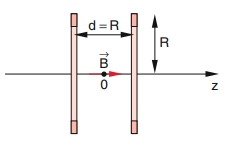
\includegraphics[]{./abbildungen/Anordnung Helmholtz.png}%
    \caption{Die Anordnung eines Helmholtz-Spulenpaars.}%
    \label{fig:Anordnung_Helmholtz}%
    \end{subfigure}%
    \hfill% Fills available space in the center -> space between figures
    \begin{subfigure}{0.48\textwidth}%
    \centering%
    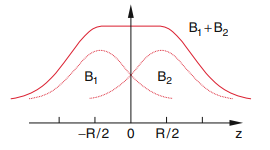
\includegraphics[]{./abbildungen/Magnetfeld Helmholtz.png}%
    \caption{Das Magnetfeld eines Helmholtz-Spulenpaars.}%
    \label{fig:Magnetfeld_Helmholtz}%
    \end{subfigure}%
    \caption{Darstellung eines Helmholtz-Spulenpaars  \cite[S.92]{demtroeder2}.}%
    \label{fig:logos}%
\end{figure}%
%
Wird Gleichung \eqref{eq:helmholtz_mitte} nach $z$ differenziert, ergibt sich der Feldgradient
\begin{align}
    \label{eq:feldgradient}
    \frac{\diff{B}}{\diff{z}} = -3 n \mu_0 I R^2 \frac{z}{\left(R^2 + z^2\right)^{5/2}}
\end{align}
entlang der Symmertrieachse.
Idealerweise ist der Feldgradient vernachlässigbar klein für einen großen Bereich, 
sodass sich näherungsweise ein homogenes Feld ergibt.

